\documentclass{beamer}
\usepackage{times}
\usepackage{tikz}
\usepackage{beamerthemesplit}
\usepackage{tcolorbox}
\usepackage{subfigure}

\title{A Tutorial of White-Box Cryptography \\ Chapter 3 Implementations}
\author{Zheng Gong\inst{1,2}\\ \url{cis.gong@gmail.com}}
\institute{\inst{1}{School of Computer Science, South China Normal University} \\ \inst{2}{Mobile Applications And Security Engineering Center of Guangdong Province}}

\date{\today}

\begin{document}

\frame
{
 \titlepage
}

\section[Outline]{}
\frame{\tableofcontents}

\section{White-box DES}
\frame
{
  \frametitle{Chow et al.'s white-box DES}

\begin{itemize}
\item At ACM DRM 2002, Chow et al. proposed a white-box DES implementation for DRM applications.
\item The terminology and notation of this implementation are inherited in the following schemes.
\item In this very beginning paper of white-box cryptography, Chow \textit{et al.} use \textit{locally secure} to illustrate the protection of key extraction with the Man-At-The-End attack.
\end{itemize}

\begin{center}
\begin{tikzpicture}
    \node[anchor=south west,inner sep=0] (image) at (0,0) { 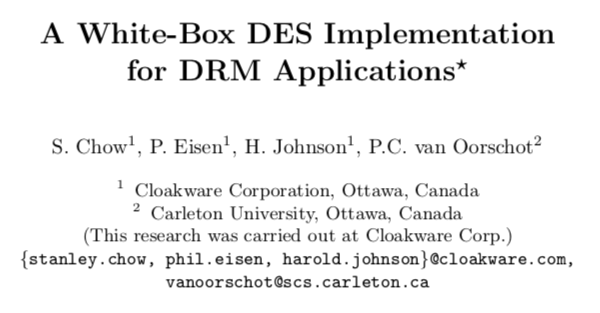
\includegraphics[width=7cm, height=3.5cm]{./pics/WBC_DES_2002.png}};

    %\begin{scope}[x={(image.south east)},y={(image.north west)}]
        %\draw[help lines,xstep=.1,ystep=.1] (0,0) grid (1,1);
        %\foreach \x in {0,1,...,9} { \node [anchor=north] at (\x/10,0) {0.\x}; }
        %\foreach \y in {0,1,...,9} { \node [anchor=east] at (0,\y/10) {0.\y}; }
        %\draw[green, ultra thick, rounded corners] (0.24,0.18) rectangle (0.50,0.32);
    %\end{scope}
\end{tikzpicture}
\end{center}
}

\subsection{Terminology and Notion}

\frame
{
\frametitle{The main concept of encoding}
For linear transformation, there are three kinds of encoding terms to obscure the intermediate values of round function.
\newline
\begin{itemize}
\item encoding

\item concatenated encoding

\item networked encoding
\end{itemize}
}

\frame
{
\frametitle{Encoding}
\begin{definition}{\textbf{(encoding)}}
Let $X$ be a transformation from $m$ to $n$ bits. Choose an $m$-bit bijection $F$ and an $n$-bit bijection $G$. Call $X^{'}=G \circ X \circ F^{-1}$ an encoded version of $X$. $F$ is an input encoding and G is an output encoding.
\end{definition}
}

\frame
{
\frametitle{Concatenated encoding}
\begin{definition}{\textbf{(concatenated encoding)}}
Consider bijection $F_{i}$ of size $n_{i}$, where $n_{1} + n_{2} + \cdots + n_{k}=n$. Let $||$ denote vector concatenation.
The function concatenation $F_{1}||F_{2}||\cdots||F_{k}$ is the bijection F such that, for any $n$-bit vector $b = (b_{1}, b_{2}, \cdots, b_{n})$, $F(b) = F_{1}(b_{1}, \cdots, b_{n_{1}})||F_{2}(b_{n_{1}+1}, \cdots, b_{n_{1}+n_{2}})||\cdots||F_{k}(b_{n+1}+\cdots+n_{k-1}, \cdots, b_{n})$. For such a bijection $F$, plainly $F^{-1} = F^{-1}_{1}||F^{-1}_{2}||\cdots||F^{-1}_{k}$.
\end{definition}

}

\frame
{
\frametitle{Networked encoding}
\begin{definition}{\textbf{networked encoding}}
A network encoding for computing $Y \circ X$ (i.e., transformation $X$ followed by transformation $Y$) is an encoding of the form:
\[Y^{'} \circ X^{'} = (H \circ Y \circ G^{-1}) \circ (G \circ X \circ F^{-1}) = H \circ (Y \circ X) \circ F^{-1}.\]
\end{definition}

}

\frame
{
\frametitle{Entropy-transference function}
$^{n}_{m}E$ is an \textit{entropy-transference function} such that $^{n}_{m}E$ maps $m$-bit vectors to $n$-bit vectors, when $m \leq n$ the mapping loses no bits of information, $m > n$ it loses at most $n-m$ bits.
}

\frame
{
\frametitle{affine transformation (\textbf{AT}) function}
A vector to vector transformation function $P$ which can be define for all $_{m}e$ by \[^{n}_{m}P(_{m}e)= ^{n}_{m}M_{m}\cdot e + _{n}d\], or \[P(e)=M\cdot e + d,\]
where $M$ is a constant matrix and $d$ is a constant \textit{displacement/masking/affine} vector.

We consider \textbf{ATs} over $GF(2)$. Note if $A$ and $B$ are \textbf{ATs}, so $A||B$ and $A \circ B$.
}

\frame
{
\frametitle{White-box precomputation}
\begin{itemize}
\item In the black-box model, a cryptographic function is algorithmically implemented beforehand and waits for inputs.

\item In the white-box model, the secret key is known first by the white-box tables generator (it might not be needed as server).
\end{itemize}

Two transformations are required for the white-box cryptosystems:
\begin{enumerate}
\item the white-box algorithm: transform the black-box version of algorithm into white-box version
\begin{itemize}
\item affine transformation
\item encoding
\end{itemize}
\item the white-box key tables: transform the round keys into a series of white-box key tables.
\end{enumerate}
}

\subsection{Producing encoded implementations}

\frame
{
\frametitle{Mixing bijection}
A \textit{mixing bijection} is a bijective \textbf{AT} which attempts to maximize the dependency of each output bit on all input bits.

\begin{itemize}
\item For example, a bit permutation layer $P$ might be sparse in a matrix representation (such as the $P$ layer in DES).

\item In order to diffuse more information over more bits, we can represent such a permutation $P=J \circ K$, where $J = P \circ K^{-1}$.
\end{itemize}
}

\frame
{
\frametitle{I/O-blocked encoding}
An arbitrary function $^{n}_{m}P$, where $m$ and $n$ are large, cannot simply be encoded using two arbitrary bijective encodings as $P'=G\circ P \circ F^{-1}$ using a look-up table. \newline

For example, a transformation $^{8}_{16}P$ requires $2^{8}\times 16=2^{12}$ bits (4Kb) storage, whilst $^{16}_{64}P$ requires $2^{16} \times 32=2^{21}$ bits (2Mb!).\newline

\textbf{Solution:}
\begin{itemize}
\item Let $F_{P} = (F_{1}||F_{2}||\cdots||F{j}) \circ J$ and $G_{P}=(G_{1}||G_{2}||\cdots||G_{k})\circ K$.
\item Concatenated encoding: $F_{j}$ is $^{a}_{a}F$ and $G_{k}$. is $^{b}_{b}G$.
\item $P'=G_{P}\circ P \circ F_{P}^{-1}$.
\end{itemize}
}

\frame
{
\frametitle{Combined function encoding}
For functions $P$ and $Q$ that happened to be evaluated  together, we could choose an encoding $P||Q$ such as $G\circ (P||Q) \circ F^{-1}$.\newline

For two $4$-bit sboxes $S_{1}(_{4}e)$ and $S_{2}(_{4}e)$, we can combine them together as an $8$-bit sbox $(S_{1}||S_{2})(_{8}e)$.

}

\frame
{
\frametitle{By-pass encoding}
In general, we want the implementation of each transform to have extra entropy at both the input and output, so that it is more difficult to extract the core.\newline

For a function $^{n}_{m}P$, we can put a \textit{by-pass encoding} $^{b}_{a}E$ such that $^{n+b}_{m+a}P'=G\circ (P||^{b}_{a}E)\circ F^{-1}$.
}

\frame
{
\frametitle{Split-path encoding}
Form a function $^{n}_{m}P$, we may use an encoding that is \textcolor[rgb]{1.00,0.00,0.00}{really a concatenation of two separate encodings}. That is, we define
\[^{n+k}_{m}Q(_{m}e)=P(_{m}e)||^{k}_{m}R(_{m}e)\]
The effect is that if $P$ is lossy, $Q$ may lose less information (or no information). This method is used to achieve \textcolor[rgb]{1.00,0.00,0.00}{local security} on Chow \textit{et al.}'s white-box DES.
}

\frame
{
\frametitle{Output splitting}
We can encode a function $P$ as $k \geq 2$ functions $P_{1}, P_{2}, \cdots, P_{k}$, where the encoded implementation for each part can mix in additional entropy. For example, \[^{n}_{m}P_{2}(_{m}e) =P(_{m}e) \oplus P_{1}(_{m}e)\]

}

\subsection{Wide-input encoded ATs}

\frame
{
\frametitle{Wide-input encoding}
\begin{itemize}
\item Due to the storage costs, it is impractical to improve the input-size of an sbox.

\item But we can use a concatenated encoding, build a wide-input encoding for a network of sboxes.
\end{itemize}

For an sbox $S$ with $n$-bit input and output (normally 4-bit or 8-bit), we can use the following wide-input encoding method:
\[^{k\times n}_{k\times m}A \circ (S_{1}||S_{2}||\cdots||S_{k})= ^{n}_{m}A_{1} \circ S_{1}||^{n}_{m}A_{2} \circ S_{2}||\cdots||^{n}_{m}A_{k} \circ S_{k}\]
}

\frame
{
\frametitle{First step of Chow et al.'s white-box DES in two rounds}
\begin{center}
\begin{tikzpicture}
    \node[anchor=south west,inner sep=0] (image) at (0,0) { 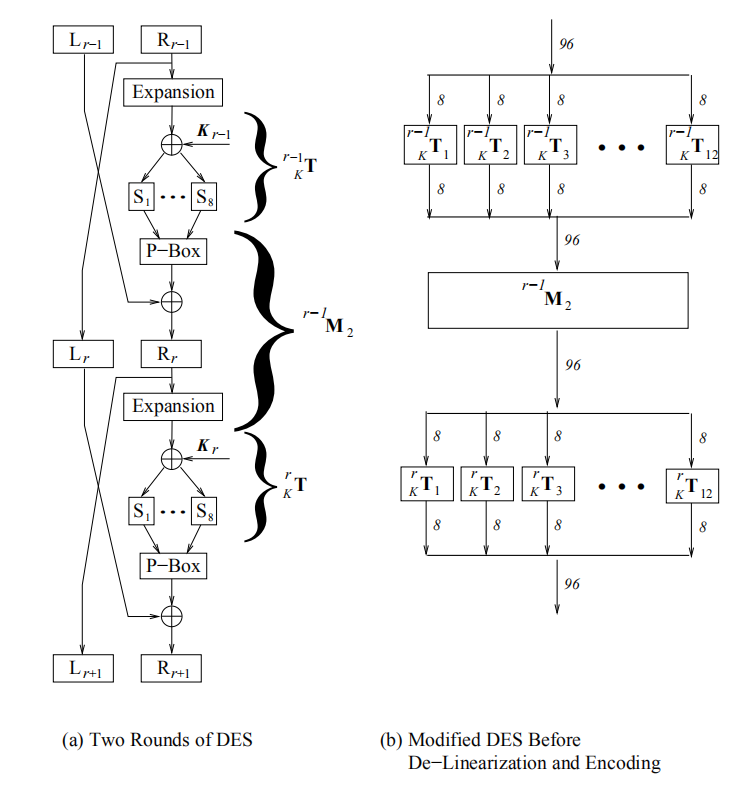
\includegraphics[width=7cm, height=7cm]{./pics/TwoRound_WBDES.png}};

    %\begin{scope}[x={(image.south east)},y={(image.north west)}]
        %\draw[help lines,xstep=.1,ystep=.1] (0,0) grid (1,1);
        %\foreach \x in {0,1,...,9} { \node [anchor=north] at (\x/10,0) {0.\x}; }
        %\foreach \y in {0,1,...,9} { \node [anchor=east] at (0,\y/10) {0.\y}; }
        %\draw[green, ultra thick, rounded corners] (0.24,0.18) rectangle (0.50,0.32);
    %\end{scope}
\end{tikzpicture}
\end{center}
}

\frame
{
\frametitle{DES sbox and its local security}
Let $6$-bit input $a=a_{0}a_{1}\cdots a_{5}$ and DES $6$-bit input and $4$-bit output sbox $^{6}_{4}S(.)$. To build a local secure look-up table $T$, we have
\[^{8}_{8}T(a||^{2}a)=^{6}_{4}S(k\oplus a)||a_{0}||a_{1}||a_{4}||a_{5}.\]

\begin{figure}[h]
\centering
\subfigure[DES 6-to-4 sbox]{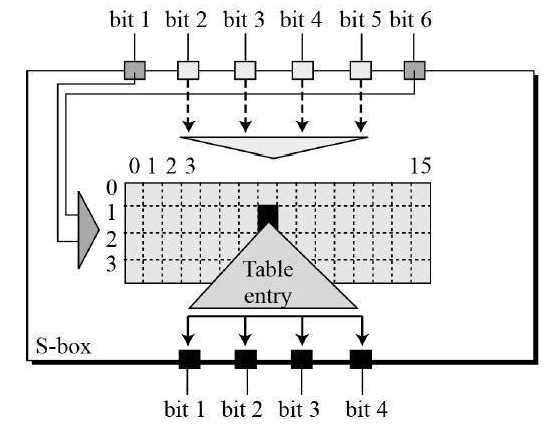
\includegraphics[width=5cm, height=4cm]{./pics/DES_Sbox.png}}
\subfigure[WBDES 8-to-8 Tbox]{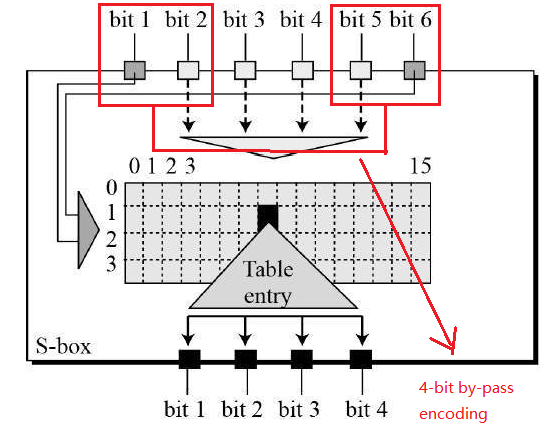
\includegraphics[width=5cm, height=4cm]{./pics/WBDES_Tbox.png}}
\end{figure}
}

\frame
{
\frametitle{(Dis)advantages of Chow \textit{et al}.'s white-box DES}
\begin{itemize}
    \item Change DES from Feistel to WBDES into a SPN structure through bypassing encoding;
    \item Modify 6-to-4-bit sboxes to 8-to-8-bit look-up tables to enhance the local security;
    \item 8-to-8-bit look-up tables are not stronger enough for resisting exhaustive search attacks;
    \item Input-output nonlinear encodings become the key point of its white-box security, yet fails in the later research.
\end{itemize}

}

\section{White-box AES}
\subsection{Chow et al.'s white-box AES}

\frame
{
\frametitle{Chow et al.'s white-box AES}
\begin{itemize}
\item At SAC 2002, Chow et al. proposed first white-box AES implementation with look-up tables.
\item The strategy is to compose each step in the AES algorithm with randomly chosen bijections, which are also called \textcolor[rgb]{1.00,0.00,0.00}{internal and external encodings}.
\end{itemize}

\begin{center}
\begin{tikzpicture}
    \node[anchor=south west,inner sep=0] (image) at (0,0) { 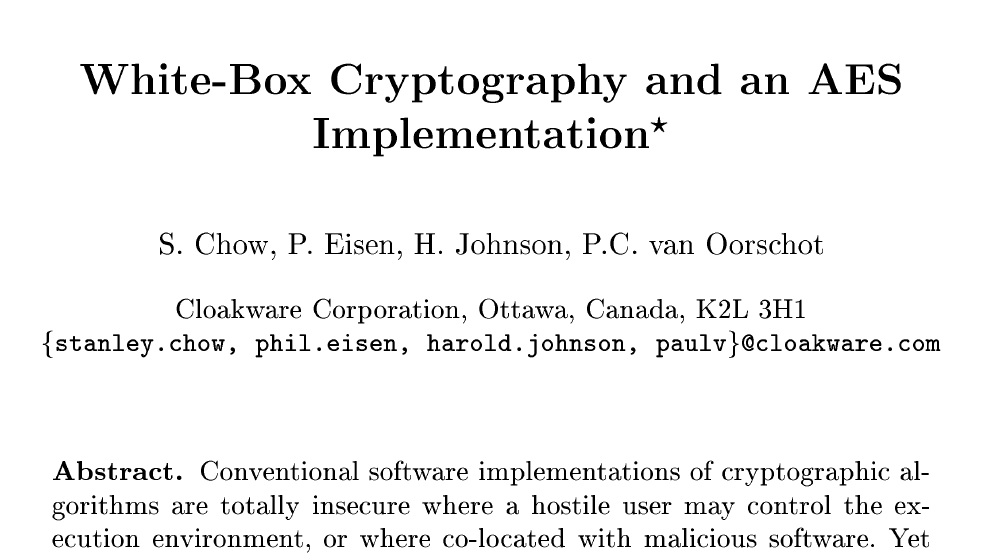
\includegraphics[width=7cm, height=3.5cm]{./pics/WBC_AES_2002.png}};

    %\begin{scope}[x={(image.south east)},y={(image.north west)}]
        %\draw[help lines,xstep=.1,ystep=.1] (0,0) grid (1,1);
        %\foreach \x in {0,1,...,9} { \node [anchor=north] at (\x/10,0) {0.\x}; }
        %\foreach \y in {0,1,...,9} { \node [anchor=east] at (0,\y/10) {0.\y}; }
        %\draw[green, ultra thick, rounded corners] (0.24,0.18) rectangle (0.50,0.32);
    %\end{scope}
\end{tikzpicture}
\end{center}
}

\frame
{
\frametitle{Fixed/Dynamic Key Approaches of WBC}
\begin{itemize}
\item \textbf{Fixed key approach}: The white-box key is fixed with the certain implementation beforehand. \textcolor[rgb]{1.00,0.00,0.00}{But it can still be changed since software is just binary.}

\item \textbf{Dynamic key approach}: The white-box key is an input encrypted/encoded value in the certain implementation, just not fixed beforehand.
\end{itemize}

No matter whether choosing fixed or dynamic key approach, the white-box instance generator takes a key and random seed(s) as input, and generates a key-customized white-box protected cipher implementation.
}

\frame
{
\frametitle{The balance between theoretical and practical white-box security}
\begin{itemize}
\item Taken to an unrealistic extreme, one could use a single look-up table of about $2^{128}\times 16$ bytes representing an AES-128 instance. But this method is impractical since it requires almost $5.4 \times 10^{39}$ bytes storage for the table.

\item Actually, all the white-box symmetric-key algorithms are trying to \textcolor[rgb]{1.00,0.00,0.00}{find the balance between the extreme case and smaller look-up tables combinations}.
\end{itemize}
}

\frame
{
\frametitle{The look-up tables of Chow \textit{et al}.'s white-box AES}
\begin{center}
\begin{tikzpicture}
    \node[anchor=south west,inner sep=0] (image) at (0,0) { 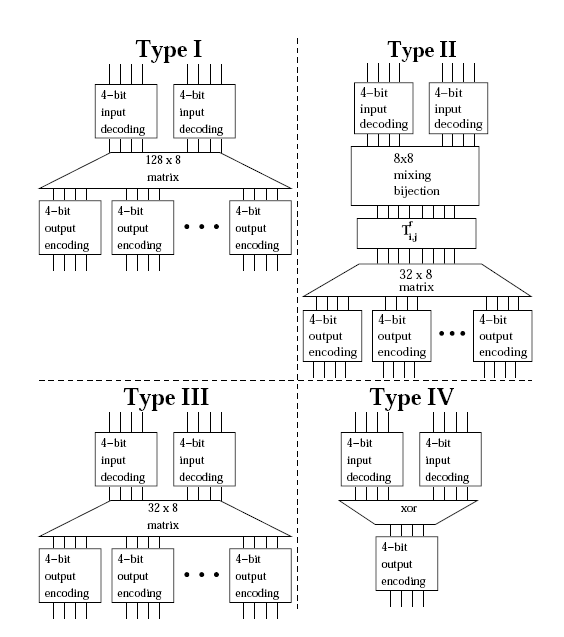
\includegraphics[width=6cm, height=6cm]{./pics/Look-up_tables_ChowWBAES}};

    %\begin{scope}[x={(image.south east)},y={(image.north west)}]
        %\draw[help lines,xstep=.1,ystep=.1] (0,0) grid (1,1);
        %\foreach \x in {0,1,...,9} { \node [anchor=north] at (\x/10,0) {0.\x}; }
        %\foreach \y in {0,1,...,9} { \node [anchor=east] at (0,\y/10) {0.\y}; }
        %\draw[green, ultra thick, rounded corners] (0.24,0.18) rectangle (0.50,0.32);
    %\end{scope}
\end{tikzpicture}
\end{center}
}

\frame
{
\frametitle{The look-up tables for the SubByte step}
For $10$ rounds AES-128, there are $16\times 10$ SubByte operations. Thus we need $160$ $8\times 8$ look-up tables to replace the SubByte operations of AES-128.
\begin{itemize}
\item From Round 1 to Round 9:
\[T^{r}_{i,j}(x)=S(x\oplus k^{r-1}_{i,j}), i,j={0,1,2,3},r={0,1,\cdots, 9}.\]

\item The final Round 10 also absorbs the post-whitening key as follows:
    \[T^{10}_{i,j}=S(x\oplus k^{9}_{i,j})\oplus k^{10}_{i,j}.\]
\end{itemize}
}

\frame
{
\frametitle{Input and output encodings}
\begin{itemize}
\item Let $X$ be a transformation from $m$ to $n$ bits.
\item Choose an $m$-bit bijection $F$ and an $n$-bit bijection $G$. The encoded version of $X$ is
  \[X' = G \circ X \circ F^{-1}.\]
\item $F$ is \textcolor[rgb]{1.00,0.00,0.00}{the input encoding} and $G$ is \textcolor[rgb]{1.00,0.00,0.00}{the output encoding}.
\item To avoid huge tables, we can construct an input or output encoding as the concatenation of smaller bijections.
\end{itemize}
}

\frame
{
\frametitle{Concatenation of encodings}
Similar to Chow \textit{et al.}'s white-box DES, results are meaningful only if the output encoding of one step matches the input encoding of the next. For example, if step $X$ is followed by step $Y$ (i.e., we compute $Y \circ X$), they are encoded as
\[Y' \circ X' = (H \circ Y \circ G^{-1}) \circ (G \circ X \circ F^{-1}) = H \circ (Y \circ X) \circ F^{-1}.\]

}

\frame
{
\frametitle{The encoded cipher $E$}
An $r$-round encryption $E_{K}=R_{1}\circ R_{2} \circ \cdots \circ R_{r}$ will be protected as an encoded version $E'_{K}$, such that
\[E'_{K}= G \circ R_{1} \circ H^{-1} \circ H \circ R_{2} \circ \cdots \circ R_{r} \circ F^{-1}=G \circ E_{K} \circ F^{-1}.\]

It is worth noting that if with any significant probability that $G \circ E_{K} \circ F^{-1}$ is weaker than $E_{K}$, then intuitively one expects the cipher $E$ is seriously flawed for key $K$ or it is weakened by the mapping functions $G$ and $F^{-1}$.
}

\frame
{
\frametitle{Min-loss encoding}
\begin{itemize}
\item If $X$ is an $n \times m$ transformation (mapping $m$ bits to $n$ bits), $m \geq n$, it will lose at least (and possible exactly) $m - n$ bits of input information.

\item However, if there are only $2^{n-k}$ possible outputs, $X$ drops $m-n+k$ bits.

\item We can hide such loss points in a look-up table network, delaying losses to later points in computation.

\item This increases the size of the attacker's search space for encodings. We call this concealment \textcolor[rgb]{1.00,0.00,0.00}{min-loss encoding}.
\end{itemize}
}

\frame
{
\frametitle{The non-linear encodings}
SubBytes+AddRoundKey+MixColumns = The non-linear encodings

\begin{figure}[h]
\setcounter{subfigure}{0}
\centering
\subfigure[MixColumns:Multiplication]{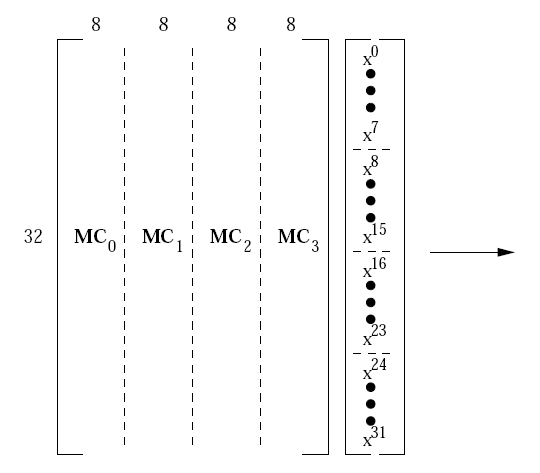
\includegraphics[width=5cm, height=4cm]{./pics/MC_MUX.png}}
\subfigure[MixColumns:Addition]{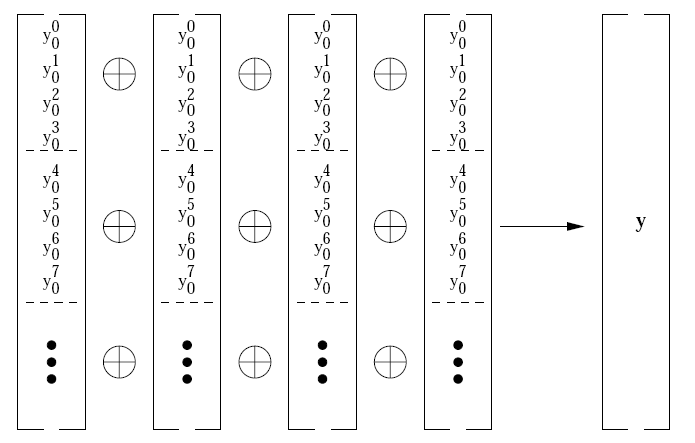
\includegraphics[width=5cm, height=4cm]{./pics/MC_ADD.png}}
\end{figure}
}

\frame
{
\frametitle{Mixing bijections}
In Chow \textit{et al.}'s white-box AES, the term \textcolor[rgb]{1.00,0.00,0.00}{mixing bijection} is used to describe a linear bijection as matrices over $GF(2)$

\begin{itemize}
\item For a $n$-bit bjiection, there are $2^{n}!$ combinations, of which $2^{n}\prod^{n-1}_{i=0}(2^{n}-2^{i})$ are affine.

\item For example, there are $16! \approx 2.09 \times 10^{13}$ 4-bit bijections of which $322,560$ (less than $0.000002\%$) are affine.
\end{itemize}
}

\frame
{
\frametitle{Mixing bijections in Chow \textit{et al.}'s WBAES}
\begin{center}
\begin{tikzpicture}
    \node[anchor=south west,inner sep=0] (image) at (0,0) { 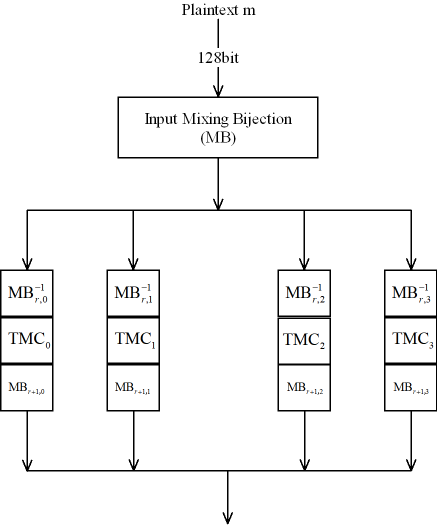
\includegraphics[width=6cm, height=7cm]{./pics/Chow_WBAES_BijectionStructure.png}};

    %\begin{scope}[x={(image.south east)},y={(image.north west)}]
        %\draw[help lines,xstep=.1,ystep=.1] (0,0) grid (1,1);
        %\foreach \x in {0,1,...,9} { \node [anchor=north] at (\x/10,0) {0.\x}; }
        %\foreach \y in {0,1,...,9} { \node [anchor=east] at (0,\y/10) {0.\y}; }
        %\draw[green, ultra thick, rounded corners] (0.24,0.18) rectangle (0.50,0.32);
    %\end{scope}
\end{tikzpicture}
\end{center}
}

\frame
{
\frametitle{Security analysis of WBAC}
\begin{itemize}
\item keyspace-like security measures:
    \begin{enumerate}
    \item white-box diversity
    \item white-box ambiguity
    \end{enumerate}

\item Cryptanalysis measures:
    \begin{enumerate}
    \item Square-like attack
    
    \end{enumerate}

\item Side-channel measures:
    \begin{enumerate}
    \item differential computation analysis
    \item differential fault analysis
    \end{enumerate}

\end{itemize}

}

\frame
{
\frametitle{White-box diversity}
\begin{itemize}
\item In a white-box block cipher algorithm, if encodings `encrypt' implementation steps, we can count the possible encoded steps. We call this metric \textcolor[rgb]{1.00,0.00,0.00}{white-box diversity}.

\item The white-box diversity of a given table type counts on how many distinct constructions exist for a table of that type, which might exceed the number of distince tables.
    
\end{itemize}
}

\frame
{
\frametitle{White-box ambiguity}
The \textcolor[rgb]{1.00,0.00,0.00}{white-box ambiguity} for a given table is the number of distinct constructions which could produce exactly that the same table.
}

\frame
{
\frametitle{The wasted step between AES and Chow \textit{et al}.'s white-box AES}


\begin{tikzpicture}
    \node[anchor=south west,inner sep=0] (image) at (0,0) { 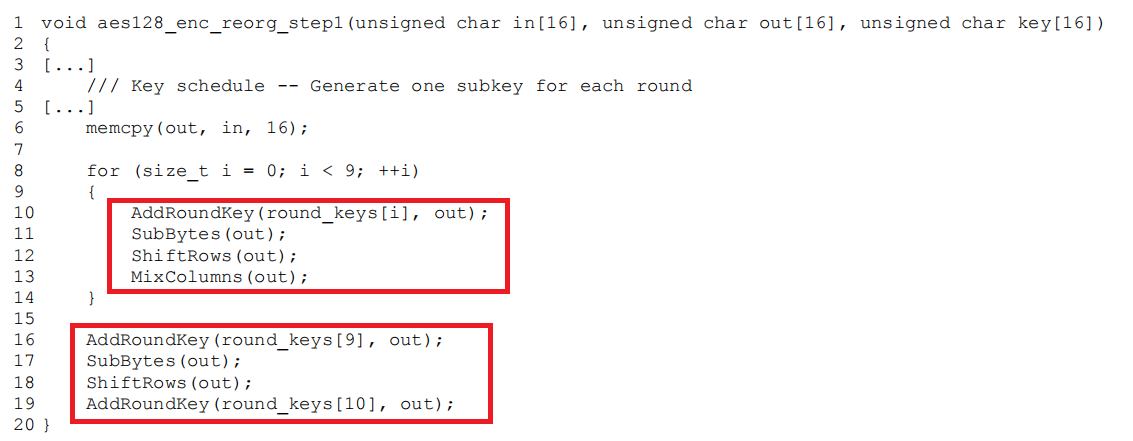
\includegraphics[width=7cm, height=3cm]{./pics/AES.png}};

    %\begin{scope}[x={(image.south east)},y={(image.north west)}]
        %\draw[help lines,xstep=.1,ystep=.1] (0,0) grid (1,1);
        %\foreach \x in {0,1,...,9} { \node [anchor=north] at (\x/10,0) {0.\x}; }
        %\foreach \y in {0,1,...,9} { \node [anchor=east] at (0,\y/10) {0.\y}; }
        %\draw[green, ultra thick, rounded corners] (0.24,0.18) rectangle (0.50,0.32);
    %\end{scope}
\end{tikzpicture}


\begin{tikzpicture}
    \node[anchor=south west,inner sep=0] (image) at (0,0) { 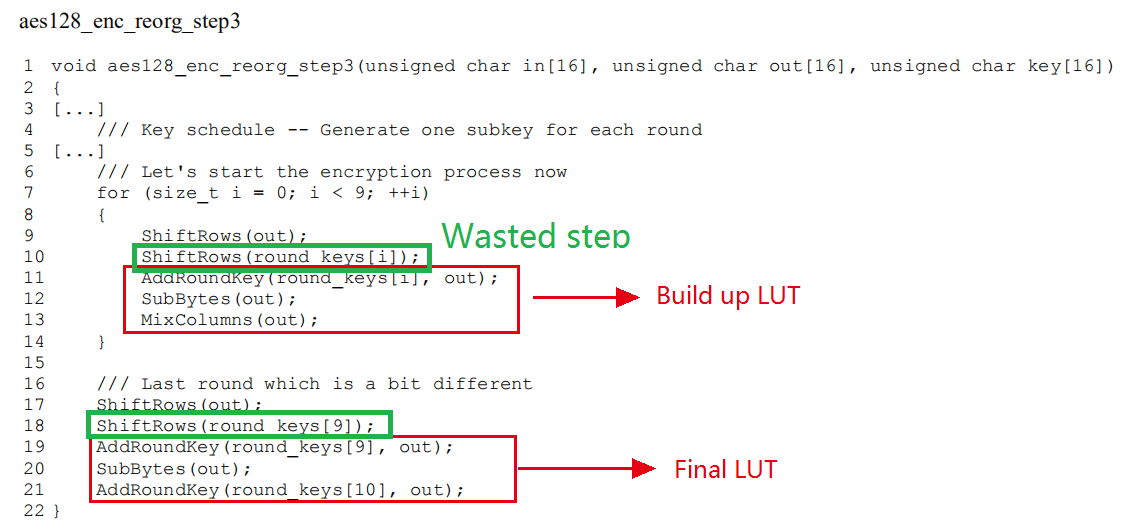
\includegraphics[width=7cm, height=3cm]{./pics/Chow_WBAES.png}};

    %\begin{scope}[x={(image.south east)},y={(image.north west)}]
        %\draw[help lines,xstep=.1,ystep=.1] (0,0) grid (1,1);
        %\foreach \x in {0,1,...,9} { \node [anchor=north] at (\x/10,0) {0.\x}; }
        %\foreach \y in {0,1,...,9} { \node [anchor=east] at (0,\y/10) {0.\y}; }
        %\draw[green, ultra thick, rounded corners] (0.24,0.18) rectangle (0.50,0.32);
    %\end{scope}
\end{tikzpicture}


}



\frame
{
\begin{center}
\textbf{Thanks for your attentions!}
\end{center}
\begin{center}
\begin{tikzpicture}
    \node[anchor=south west,inner sep=0] (image) at (0,0) { 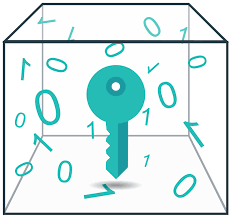
\includegraphics[width=4cm, height=4cm]{./pics/WBC_BG.png}};

    %\begin{scope}[x={(image.south east)},y={(image.north west)}]
        %\draw[help lines,xstep=.1,ystep=.1] (0,0) grid (1,1);
        %\foreach \x in {0,1,...,9} { \node [anchor=north] at (\x/10,0) {0.\x}; }
        %\foreach \y in {0,1,...,9} { \node [anchor=east] at (0,\y/10) {0.\y}; }
        %\draw[green, ultra thick, rounded corners] (0.24,0.18) rectangle (0.50,0.32);
    %\end{scope}
\end{tikzpicture}

\end{center}
}

\end{document}
